\def\mytitle{LINE ASSIGNMENT}
\def\myauthor{G.Kumar}
\def\contact{kumargandhamaneni20016@gmail.com}
\def\mymodule{Future Wireless Communication (FWC)}
\documentclass[10pt, a4paper]{article}
\usepackage[a4paper,outer=1.5cm,inner=1.5cm,top=1.75cm,bottom=1.5cm]{geometry}
\twocolumn
\usepackage{graphicx}
\graphicspath{{./images/}}
\usepackage[colorlinks,linkcolor={black},citecolor={blue!80!black},urlcolor={blue!80!black}]{hyperref}
\usepackage[parfill]{parskip}
\usepackage{lmodern}
\usepackage{tikz}
\usepackage{physics}
\usepackage{tabularx}
\usetikzlibrary{calc}
\usepackage{amsmath}
\usepackage{amssymb}
\renewcommand*\familydefault{\sfdefault}
\usepackage{watermark}
\usepackage{lipsum}
\usepackage{xcolor}
\usepackage{listings}
\usepackage{float}
\usepackage{titlesec}
\providecommand{\mtx}[1]{\mathbf{#1}}
\titlespacing{\subsection}{1pt}{\parskip}{3pt}
\titlespacing{\subsubsection}{0pt}{\parskip}{-\parskip}
\titlespacing{\paragraph}{0pt}{\parskip}{\parskip}
\newcommand{\figuremacro}[5]{
    \begin{figure}[#1]
        \centering
        \includegraphics[width=#5\columnwidth]{#2}
        \caption[#3]{\textbf{#3}#4}
        \label{fig:#2}
    \end{figure}
}
\newcommand{\myvec}[1]{\ensuremath{\begin{pmatrix}#1\end{pmatrix}}}
\let\vec\mathbf
\lstset{
frame=single, 
breaklines=true,
columns=fullflexible
}
\thiswatermark{\centering \put(0,-105.0){
\includegraphics[scale=0.35]{iith}} }
\title{\mytitle}
\author{\myauthor\hspace{1em}\\\contact\\IITH\hspace{0.5em}-\hspace{0.5em}\mymodule}
\date{}
\begin{document}
	\maketitle
\section*{Problem}
   Find angle between the lines,$\sqrt{3}$x+y=1 and x+$\sqrt{3}$y=1.
   \section*{Solution}
   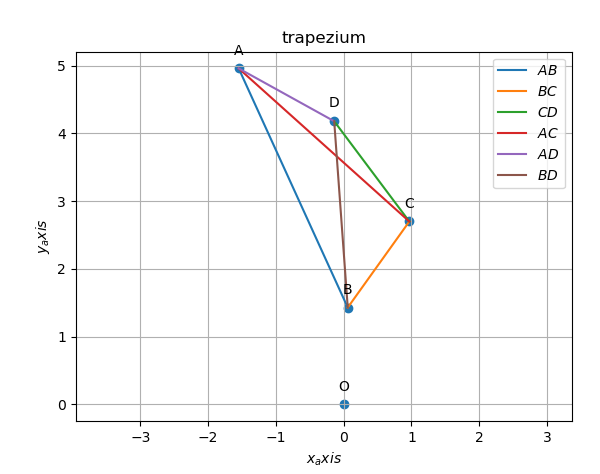
\includegraphics[scale=0.55]{line.png}
   The input parameters for this construction are :
   \begin{center}
\begin{tabular}{|c|c|c|}
	\hline
	\textbf{Symbol}&\textbf{Value}&\textbf{Description}\\
	\hline
	P&$\
	\begin{pmatrix}
		0.57736 \\
		0 \\
	\end{pmatrix}$%
	&Point P\\ 
	\hline
	X&$\
	\begin{pmatrix}
		0.36603 \\
		0.36603 \\
	\end{pmatrix}$%
	&Point X\\
	\hline
	Q&$\
	\begin{pmatrix}
		1 \\
		0 \\
	\end{pmatrix}$%
	&Point Q\\
	
	\hline
\end{tabular}
\end{center}
   \subsection*{Step 1}
   Given two equations are, \\
   \begin{equation}
   \sqrt{3}x+y=1 
   \end{equation}
   \begin{equation}
   x+\sqrt{3}y=1 
   \end{equation}
   Equation(1) in vector form is given as,
   \begin{align}
   \myvec{\sqrt{3}&1}\vec{x}=1
   \end{align}
   From this, Normal vector to the line is given as,
   \begin{align*}
   \vec{n_1}=\myvec{\sqrt{3}\\1}
   \end{align*}
   So, the direction vector of the line is given as,
\begin{eqnarray*}
   \vec{m1}=\myvec{-1\\\sqrt{3}}
\end{eqnarray*} 
Similarly, Normal vector to the line(2) is given as,
   \begin{align*}
   \vec{n_2}=\myvec{1\\\sqrt{3}}
   \end{align*}
   So, the direction vector of the line is given as,
\begin{eqnarray*}
   \vec{m2}=\myvec{-\sqrt{3}\\1}
\end{eqnarray*}     

\subsection*{Step 2}
Now, Angle between any two lines,using their direction vectors, is given by, \\
\begin{eqnarray*}
 cos\theta=\frac{(\vec{m1})^T(\vec{m2})}{\norm{\vec{m1}}\norm{\vec{m2}}}
\end{eqnarray*}
So, Angle between the two lines is given by,
\begin{eqnarray}
 cos\angle{x}=\frac{(\vec{m1})^T(\vec{m2})}{\norm{\vec{m1}}\norm{\vec{m2}}}\
\end{eqnarray}
\begin{eqnarray}
 cos\angle{x}=\frac{\myvec{-1\\\sqrt{3}}^T\myvec{-\sqrt{3}\\1}}{\norm{\myvec{-1\\\sqrt{3}}}\norm{\myvec{-\sqrt{3}\\1}}}
\end{eqnarray}
By solving the above equation, we get, \\
\begin{equation}
cos\angle{x}=\frac{\sqrt{3}}{2} \\
\end{equation}
This Implies,
\begin{equation*}
\angle{x}=30^\circ
\end{equation*}
Therefore, the angle between given two lines is $30^\circ$. \\
\bibliographystyle{ieeetr}
\end{document}